\section{}
The figure shows a traction elevator system used in high-rise residential buildings. These traction 
elevators consist of hoist cables connected to the top of the cab operated by a traction machine 
(electric motor) located in the penthouse. The system is modelled as a simple spring-mass system, 
where the spring represents the cable stiffness and the mass corresponds to the elevator cab and its 
occupants (counterweights are neglected).
\begin{figure}[h]
    \centering
    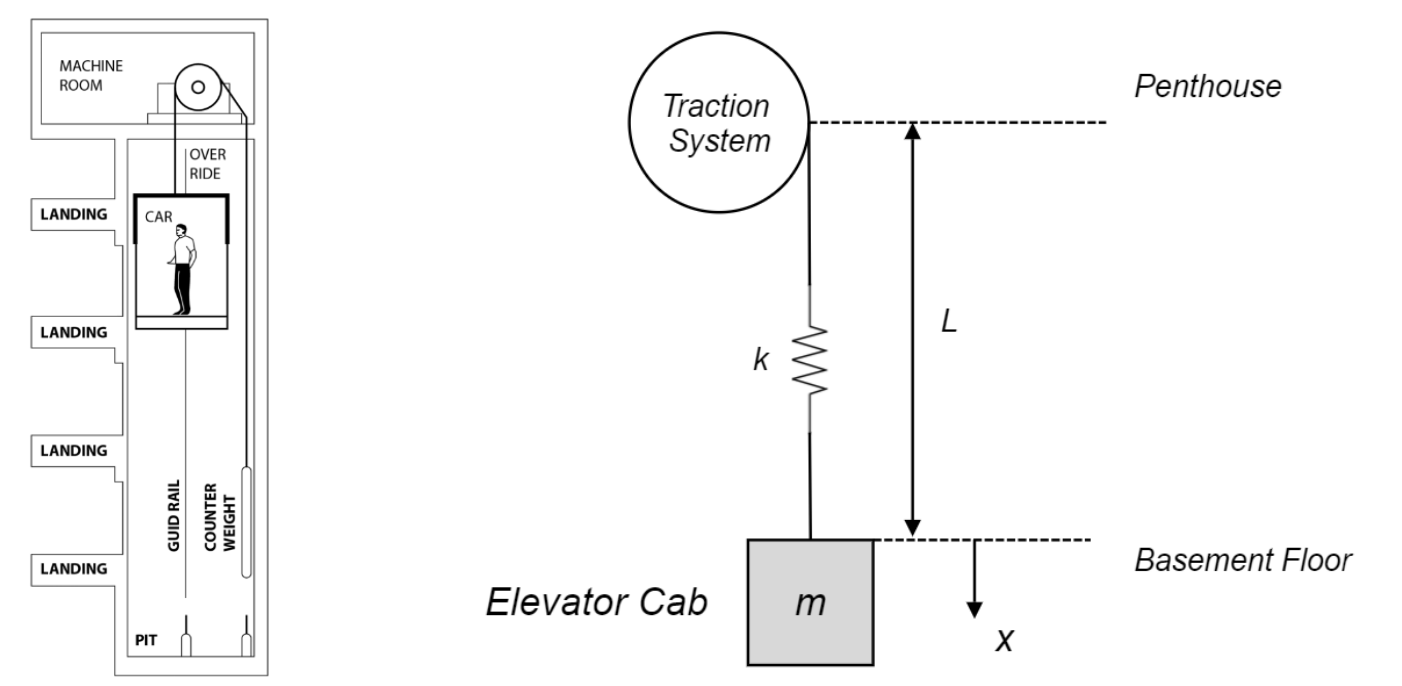
\includegraphics[width=0.5\linewidth]{Questions/Figures/q4 problem diagram.png}
    \caption{The traction elevator system}
    \label{fig:q4-png}
\end{figure}
The elevator provides a rapid ascent/descent, while not causing excessive acceleration to the
passengers or stress in the cable system. The situation under consideration is the stop after descent
to the basement floor level for a 10 floor apartment building (assume 3.5 m per story). Assume
that the traction motor stops instantly when reaching the basement floor (acts as a fixed support).
The velocity of the cab before stopping is 1.5 m/s. The cables have an equivalent stiffness of a
single cable with a radius of 2 cm and an elastic modulus of 100 GPa ($k = \frac{EA}{L}$).

\begin{enumerate}[label=(\alph*)]
    \item Consider both cases with an unloaded cab (mass of 1.2 metric tonnes) and with a maximum
        capacity of 15 people with an average weight of 70 kg each. For each case, determine:
        \begin{enumerate}[label=(\roman*)]
            \item (1 pt) The overshoot of the cab past the basement floor level after stopping.
            \item (1 pt) The maximum acceleration felt by the occupants.
            \item (1 pt) The maximum stress in the cables.
        \end{enumerate}
    \item (3 pts) To reduce the maximum tension in the cables and acceleration of the cab, a coil
        spring ($k = 600$ kN/m) is inserted between the cable attachment and the cab. How does
        this change the maximum displacement, acceleration, and stress for both the loaded and
        unloaded cases?
    \item The results for the vibration analysis of the original elevator system (no coil spring) was done
        under the assumption of no damping. However, the system components have an inherent
        damping. a test was done on an UNLOADED cab and it was found that the cab's oscillation
        amplitude decreased by 50\% in two cycles.
        \begin{enumerate}[label=(\roman*)]
            \item (2 pts) Determine the damping ratio for the LOADED case assuming viscous damping.
            \item (2 pts) For the LOADED case, estimate how much time is needed after reaching the ground
                floor so that the passengers feel virtually no vibration of the elevator cab. Assume that the
                vibrations essentially stop when the amplitude decreases to 8\% of its maximum value.
                Hint: recall that the logarithmic decrement is measured between subsequent peaks, so you
                must account for the time from $t = 0$ to the first peak.
        \end{enumerate}
\end{enumerate}

\subsection*{Solution}
\subsection{}
The system acts as a simple spring-mass system with initial conditions $x(0) = 0$ and $\dot{x}(0) = 1.5$ m/s. Assume that the equilibrium position is at the basement floor level.

The equation of motion is:
\begin{align*}
    \ddot{x} + \frac{k}{m} x &= 0
\end{align*}
with the general solution:
\begin{align*}
    x(t) &= A \cos (pt) + B \sin (pt)
\end{align*}
with the solution to the initial conditions:
\begin{align*}
    x(0) &= 0 \implies A = 0 \\
    \dot{x}(0) &= 1.5 \implies B = 1.5/p
\end{align*}
So the solution is:
\begin{align*}
    x(t) &= \frac{1.5}{p} \sin (pt)
\end{align*}
Next, the spring constant can be found by
\begin{align*}
    k &= \frac{EA}{L} = \frac{(100 \times 10^9) \pi (0.02)^2}{3.5 \times 10} = 3.59 \text{Mn/m}
\end{align*}
So the natural frequency for both cases is:
\begin{align*}
    p_{\text{unloaded}} &=  \sqrt{\frac{3.59 \times 10^6}{1200}} = 54.7 \text{rad/s} \\
    p_{\text{loaded}} &=  \sqrt{\frac{3.59 \times 10^6}{1200 + 15 \times 70}} = 39.9 \text{rad/s}
\end{align*}

The overshoot of the cab is simply the amplitude of the solution. So,
\begin{empheq}[box=\fbox]{align*}
    x_{\text{unloaded}, \text{overshoot}} &= \frac{1.5}{54.7} = 0.0274 \text{m} \\
    x_{\text{loaded}, \text{overshoot}} &= \frac{1.5}{39.9} = 0.0376 \text{m}
\end{empheq}

To find the maximum acceleration, we can take the second derivative of the solution 
\begin{align*}
    \ddot{x} &= -1.5 p \cos (pt)
\end{align*}
The maximum acceleration is the amplitude of the second derivative. So,
\begin{empheq}[box=\fbox]{align*}
    \ddot{x}_{\text{unloaded}, \text{max}} &= 1.5 \times 54.7 = 82.0 \text{m/s}^2 \\
    \ddot{x}_{\text{loaded}, \text{max}} &= 1.5 \times 39.9 = 59.9 \text{m/s}^2
\end{empheq}
The maximum stress in the cables is at the maximum displacement. So,
\begin{align*}
    \sigma_{\text{max}} &= \frac{k}{A} x_{\text{max}}  
\end{align*}
\begin{empheq}[box=\fbox]{align*}
    \implies \sigma_{\text{unloaded}, \text{max}} &= \frac{3.59 \times 10^6}{\pi (0.02)^2} \times 0.0274 = 78.35 \text{MPa} \\
    \implies \sigma_{\text{loaded}, \text{max}} &= \frac{3.59 \times 10^6}{\pi (0.02)^2} \times 0.0376 = 107.3 \text{MPa}
\end{empheq}

\subsection{}
An additional spring is added in series with the cable. For a simple oscillator, as seen in the Effective Stiffness Examples.pdf, the effective stiffness is given by:
\begin{align*}
    k_{\text{eff}} &= \frac{k_1 k_2}{k_1 + k_2}
\end{align*}
So the effective stiffness is:
\begin{align*}
    k_{\text{eff}} &= \frac{3.59 \times 10^6 \times 600 \times 10^3}{3.59 \times 10^6 + 600 \times 10^3} = 0.514 \text{Mn/m}
\end{align*}
So the new natural frequency for both cases is:
\begin{align*}
    p_{\text{unloaded}} &=  \sqrt{\frac{0.514 \times 10^6}{1200}} = 20.70 \text{rad/s} \\
    p_{\text{loaded}} &=  \sqrt{\frac{0.514 \times 10^6}{1200 + 15 \times 70}} = 15.1 \text{rad/s}
\end{align*}
The overshoot of the cab is 
\begin{empheq}[box=\fbox]{align*}
    x_{\text{unloaded}, \text{overshoot}} &= \frac{1.5}{20.70} = 0.0725 \text{m} \\
    x_{\text{loaded}, \text{overshoot}} &= \frac{1.5}{15.1} = 0.0993 \text{m}
\end{empheq}
The maximum acceleration is
\begin{empheq}[box=\fbox]{align*}
    \ddot{x}_{\text{unloaded}, \text{max}} &= 1.5 \times 20.70 = 31.1 \text{m/s}^2 \\
    \ddot{x}_{\text{loaded}, \text{max}} &= 1.5 \times 15.1 = 22.7 \text{m/s}^2
\end{empheq}
The maximum stress in the cables is at the maximum displacement. So,
\begin{align*}
    \sigma_{\text{max}} &= \frac{k}{A} x_{\text{max}}
\end{align*}
\begin{empheq}[box=\fbox]{align*}
    \implies \sigma_{\text{unloaded}, \text{max}} &= \frac{0.514 \times 10^6}{\pi (0.02)^2} \times 0.0725 = 29.7 \text{MPa} \\
    \implies \sigma_{\text{loaded}, \text{max}} &= \frac{0.514 \times 10^6}{\pi (0.02)^2} \times 0.0993 = 40.6 \text{MPa}
\end{empheq}

\subsection{}
Using the unloaded system, the damping ratio can be found through the logarithmic decrement (eq. 3.19).
\begin{align*}
    \delta &= \ln\left(\frac{x_1}{x_2}\right) \\
    \zeta &= \frac{\delta}{\sqrt{4\pi^2 + \delta^2}}
\end{align*}
where $x_1$ and $x_2$ are the amplitudes of the first and second peaks respectively. So then,
\begin{align*}
    \delta &= \ln\left(\frac{0.0274}{0.0274 \times 0.5}\right) = 0.6931 \\
    \zeta &= \frac{0.6931}{\sqrt{4\pi^2 + 0.6931^2}} = 0.1096 
\end{align*}
From the definition of the damping ratio, 
\begin{align*}
    \zeta &= \frac{c}{2mp}
\end{align*}
So the damping coefficient is:
\begin{align*}
    c &= 2mp\zeta = 2 \times 1200 \times 54.7 \times 0.1096 = 14388.3 \text{N s/m}
\end{align*}
Calculating the damping ratio for the loaded case,
\begin{empheq}[box=\fbox]{align*}
    \zeta &= \frac{c}{2mp} \\
    &= \frac{14388.3}{2 \times (1200 + 15 \times 70) \times 39.9} \\
    &= 0.0801
\end{empheq}

\subsection{}
For the time to reach 8\% of the maximum amplitude, (eq. 3.20) can be used to find the time from the zeroth peak to the m-th peak.
\begin{align*}
    \frac{\ln(x_n / x_{n+m}) \sqrt{1 - \zeta^2}}{2\pi\zeta} &= m 
\end{align*}
then let $x_n/x_{n+m} = 1/0.08 = 12.5$. So,
\begin{align*}
    m &= \frac{\ln(12.5) \sqrt{1 - 0.0801^2}}{2\pi \times 0.0801} = 5.00
\end{align*}
so the time can be found by
\begin{align*}
    \Aboxed{t &= m \tau = 5 \times \frac{2\pi}{\sqrt{1- \zeta^2}p} = 5 \times \frac{2\pi}{\sqrt{1- 0.0801^2} \times 39.9} = 0.790 \text{s}}
\end{align*}
